\hypertarget{sec:AMK-Results}{%
\section{Results}\label{sec:AMK-Results}}

\hypertarget{the-ground-state-flux-sector}{%
\subsection{The Ground State Flux Sector}\label{the-ground-state-flux-sector}}

Here I will discuss the numerical evidence that our guess for the ground state flux sector is correct. We will do this by enumerating all the flux sectors of many separate system realisations. However there are some issues we will need to address to make this argument work.

We have two seemingly irreconcilable problems. Finite size effects have a large energetic contribution for small systems~\autocite{kitaevAnyonsExactlySolved2006} so we would like to perform our analysis for very large lattices. However for an amorphous system with \(N\) plaquettes, \(2N\) edges and \(3N\) vertices we have \(2^{N-1}\) flux sectors to check and diagonalisation scales with \(\mathcal{0}(N^3)\). That exponential scaling makes it infeasible to work with lattices much larger than \(16\) plaquettes.

To get around this we instead look at periodic systems with amorphous unit cells. For a similarly sized periodic system with \(A\) unit cells and \(B\) plaquettes in each unit cell where \(N \sim AB\) things get much better. We can use Bloch's theorem to diagonalise this system in about \(\mathcal{0}(A B^3)\) operations, and more importantly there are only \(2^{B-1}\) flux sectors to check.

We fully enumerated the flux sectors of \textasciitilde25,000 periodic systems with disordered unit cells of up to \(B = 16\) plaquettes and \(A = 100\) unit cells.

However, showing that our guess is correct for periodic systems with disordered unit cells is not quite convincing on its own. We have effectively removed longer-range disorder from our lattices.

The second part of the argument is to show that the energetic effect of introducing periodicity scales away as we go to larger system sizes and has already diminished to a small enough value at 16 plaquettes, which is indeed what we find.

From this we argue that the results for small periodic systems generalise to large amorphous systems. We perform this analysis for both the isotropic point (\(J^\alpha = 1\)), as well as in the toric code phase (\(J^x = J^y = 0.25, J^z = 1\)).

In the isotropic case (\(J^\alpha = 1\)), our conjecture correctly predicted the ground state flux sector for all of the lattices we tested.

For the toric code phase (\(J^x, J^y = 0.25, J^z = 1\)) all but around (\(\sim 0.5 \%\)) lattices had ground states conforming to our conjecture. In these cases, the energy difference between the true ground state and our prediction was on the order of \(10^{-6} J\). It is unclear whether this is a finite size effect or something else.

\hypertarget{spontaneous-chiral-symmetry-breaking}{%
\subsection{Spontaneous Chiral Symmetry Breaking}\label{spontaneous-chiral-symmetry-breaking}}

The spin Kitaev Hamiltonian is real and therefore has time reversal symmetry (TRS). However, the flux \(\phi_p\) through any plaquette with an odd number of sides has imaginary eigenvalues \(\pm i\). The ground state sector induces a relatively regular pattern for the imaginary fluxes with only a global two-fold chiral degeneracy.

Thus, states with a fixed flux sector spontaneously break time reversal symmetry. This was first described by Yao and Kivelson~for a translation invariant Kitaev model with odd sided plaquettes~\autocite{Yao2011}.

So we have flux sectors that come in degenerate pairs, where time reversal is equivalent to inverting the flux through every odd plaquette, a general feature for lattices with odd plaquettes~\autocite{yaoExactChiralSpin2007,Peri2020}. This spontaneously broken symmetry avoids the need to explicitly break TRS with a magnetic field term as is done in the original honeycomb model.

\hypertarget{ground-state-phase-diagram}{%
\subsection{Ground State Phase Diagram}\label{ground-state-phase-diagram}}

As previously discussed, the standard Honeycomb model has a Abelian, gapped phase in the anisotropic region (the A phase) and is gapless in the isotropic region. The introduction of a magnetic field breaks the chiral symmetry, leading to the isotropic region becoming a gapped, non-Abelian phase, the B phase.

We set the energy scale by requiring that \(J_x + J_y + J_z = 1\), this restricts the 3D phase space down to an equilateral triangle that is convenient for diagrams. Imagine the cube defined by \(J_\alpha \in [0,1]\) being cut by the plane \(J_x + J_y + J_z = 1\), we plot the projection of that plane in diagrams like \cref{fig:phase_diagram}.

Similar to the Kitaev Honeycomb model with a magnetic field, we find that the amorphous model is only gapless along critical lines, see \cref{fig:phase_diagram} (Left).

Interestingly, the gap closing exists in only one of the four topological sectors, though this is certainly a finite size effect as the sectors must become degenerate in the thermodynamic limit. Nevertheless this could be a useful way to define the (0, 0) topological flux sector for the amorphous model.

In the honeycomb model, the phase boundaries are located on the straight lines \(|J^x| = |J^y| + |J^x|\) and permutations of \(x,y,z\), shown as dotted line on \textasciitilde{}\ref{fig:phase_diagram} (Right). We find that on the amorphous lattice these boundaries exhibit an inward curvature, similar to honeycomb Kitaev models with flux~\autocite{Nasu_Thermal_2015} or bond~\autocite{knolle_dynamics_2016} disorder.

\hypertarget{fig:phase_diagram}{%
\begin{figure}
\centering
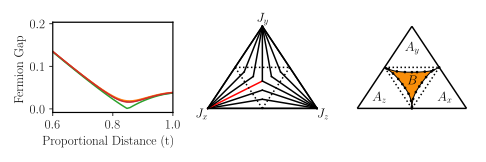
\includegraphics[width=1\textwidth,height=\textheight]{figure_code/amk_chapter/results/phase_diagram/phase_diagram}
\caption[{The Ground State Phase Diagram}]{(Center) We choose an energy scale for the Hamiltonian by setting \(J_x + J_y + J_z = 1\). This intersects a plane with the unit cube spanned by \(J_\alpha \in [0,1]\), giving a triangle with corners \((1,0,0), (0,1,0), (0,0,1)\). To compute critical lines efficiently in this space we evaluate the order parameter of interest along rays shooting from the corners. The ray highlighted in red defines the values of J used for the left figure. (Left) The fermion gap as a function of J for an amorphous system with 20 plaquettes, where the x axis is the position on the red line in the central figure from 0 to 1. For finite size systems the four topological sectors are not degenerate and only one of them has a true gap closing. (Right) The Abelian \(A_\alpha\) phases of the model and the non-Abelian B phase separated by critical lines where the fermion gap closes. Later we will show that the Chern number \(\nu\) changes from \(0\) to \(\pm 1\) from the A phases to the B phase. Indeed the gap \emph{must} close in order for the Chern number to change \textbf{citation}.}
\label{fig:phase_diagram}
\end{figure}
}

\hypertarget{is-it-abelian-or-non-abelian}{%
\subsubsection{Is it Abelian or non-Abelian?}\label{is-it-abelian-or-non-abelian}}

The two phases of the amorphous model are clearly gapped, though later I'll double check this with finite size scaling.

The next question is: do these phases support excitations with Abelian or non-Abelian statistics? To answer that we turn to Chern numbers~\autocite{berryQuantalPhaseFactors1984,simonHolonomyQuantumAdiabatic1983,thoulessQuantizedHallConductance1982}. As discussed earlier the Chern number is a quantity intimately linked to both the topological properties and the anyonic statistics of a model. Here we will make use of the fact that the Abelian/non-Abelian character of a model is linked to its Chern number \textbf{{[}citation{]}}. However the Chern number is only defined for the translation invariant case because it relies on integrals defined in k-space.

A family of real space generalisations of the Chern number that work for amorphous systems exist called local topological markers~\autocite{bianco_mapping_2011,Hastings_Almost_2010,mitchellAmorphousTopologicalInsulators2018} and indeed Kitaev defines one in his original paper on the model~\autocite{kitaevAnyonsExactlySolved2006}.

Here we use the crosshair marker of~\autocite{peru_preprint} because it works well on smaller systems. We calculate the projector \(P = \sum_i |\psi_i\rangle \langle \psi_i|\) onto the occupied fermion eigenstates of the system in open boundary conditions. The projector encodes local information about the occupied eigenstates of the system and is typically exponentially localised \textbf{{[}cite{]}}. The name \emph{crosshair} comes from the fact that the marker is defined with respect to a particular point \((x_0, y_0)\) by step functions in x and y

\[\begin{aligned}
    \nu (x, y) = 4\pi \; \Im\; \mathrm{Tr}_{\mathrm{B}} 
    \left ( 
    \hat{P}\;\hat{\theta}(x-x_0)\;\hat{P}\;\hat{\theta}(y-y_0)\; \hat{P}
    \right ),
\end{aligned}\]

when the trace is taken over a region \(B\) around \((x_0, y_0)\) that is large enough to include local information about the system but does not come too close to the edges. If these conditions are met then then this quantity will be very close to quantised to the Chern number, see \cref{fig:phase_diagram_chern}.

We'll use the crosshair marker to assess the Abelian/non-Abelian character of the phases.

In the A phase of the amorphous model we find that \(\nu=0\) and hence the excitations have Abelian character, similar to the honeycomb model. This phase is thus the amorphous analogue of the Abelian toric-code quantum spin liquid~\autocite{kitaev_fault-tolerant_2003}.

The B phase has \(\nu=\pm1\) so is a non-Abelian \emph{chiral spin liquid} (CSL) similar to that of the Yao-Kivelson model~\autocite{yaoExactChiralSpin2007}. The CSL state is the the magnetic analogue of the fractional quantum Hall state \textbf{{[}cite{]}}. Hereafter we focus our attention on this phase.

\hypertarget{fig:phase_diagram_chern}{%
\begin{figure}
\centering
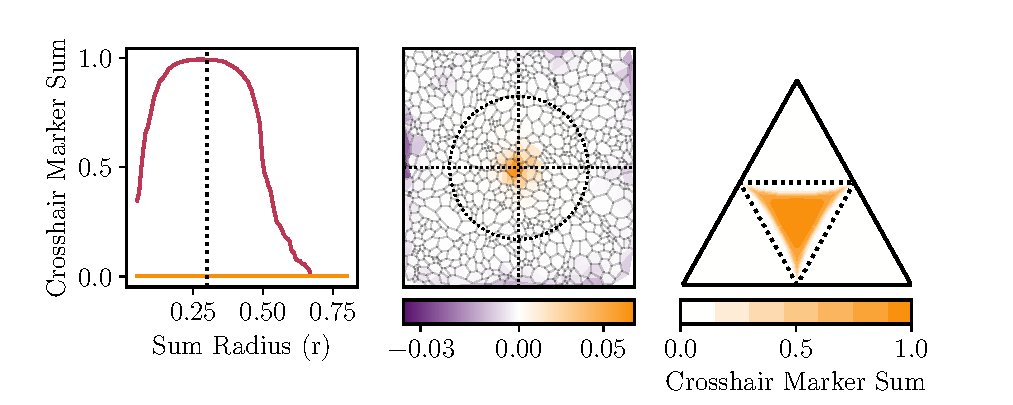
\includegraphics[width=1\textwidth,height=\textheight]{figure_code/amk_chapter/results/phase_diagram_chern/phase_diagram_chern}
\caption[{Local Chern Markers}]{(Center) The crosshair marker~\autocite{peru_preprint}, a local topological marker, evaluated on the Amorphous Kitaev Model. The marker is defined around a point, denoted by the dotted crosshair. Information about the local topological properties of the system are encoded within a region around that point. (Left) Summing these contributions up to some finite radius (dotted line here, dotted circle in the centre) gives a generalised version of the Chern number for the system which becomes quantised in the thermodynamic limit. The radius must be chosen large enough to capture information about the local properties of the lattice while not so large as to include contributions from the edge states. The isotropic regime \(J_\alpha = 1\) in red has \(\nu = \pm 1\) implying it supports excitations with non-Abelian statistics, while the anisotropic regime in orange has \(\nu = \pm 0\) implying it has Abelian statistics. (Right) Extending this analysis to the whole \(J_\alpha\) phase diagram with fixed \(r = 0.3\) nicely confirms that the isotropic phase is non-Abelian.}
\label{fig:phase_diagram_chern}
\end{figure}
}

\hypertarget{edge-modes}{%
\subsubsection{Edge Modes}\label{edge-modes}}

Chiral Spin Liquids support topological protected edge modes on open boundary conditions~\autocite{qi_general_2006}. \cref{fig:edge_modes} shows the probability density of one such edge mode. It is near zero energy and exponentially localised to the boundary of the system. While the model is gapped in periodic boundary conditions (i.e on the torus) these edge modes appear in the gap when the boundary is cut.

The localization of the edge modes can be quantified by their inverse participation ratio (IPR), \[\mathrm{IPR} = \int d^2r|\psi(\mathbf{r})|^4  \propto L^{-\tau},\] where \(L\sim\sqrt{N}\) is the linear dimension of the amorphous lattices and \(\tau\) the dimensional scaling exponent of IPR. This is relevant because localised in-gap states do not participate in transport and hence do not turn band insulators into metals. It is only when the gap fills with extended states that we get a metallic state.

\hypertarget{fig:edge_modes}{%
\begin{figure}
\centering
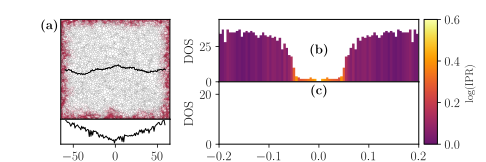
\includegraphics[width=1\textwidth,height=\textheight]{figure_code/amk_chapter/results/edge_modes/edge_modes}
\caption[{Edges States and Density of States}]{(a) The density of one of the topologically protected edge states in the B phase. (Below) the log density plotted along the black path showing that the state is exponentially localised. (a)/(b) The density of states of the corresponding lattice in (a) periodic boundary conditions, (b) open boundary conditions. The colour of the bars shows the mean log IPR for each energy window. Cutting the boundary fills the gap with localised states.}
\label{fig:edge_modes}
\end{figure}
}

\hypertarget{anderson-transition-to-a-thermal-metal}{%
\subsection{Anderson Transition to a Thermal Metal}\label{anderson-transition-to-a-thermal-metal}}

Previous work on the honeycomb model at finite temperature has shown that the B phase undergoes a thermal transition from a quantum spin liquid phase a to a \textbf{thermal metal} phase~\autocite{selfThermallyInducedMetallic2019}.

This happens because at finite temperature, thermal fluctuations lead to spontaneous vortex-pair formation. As discussed previously these fluxes are dressed by Majorana bounds states and the composite object is an Ising-type non-Abelian anyon~\autocite{Beenakker2013}. The interactions between these anyons are oscillatory similar to the RKKY exchange and decay exponentially with separation~\autocite{Laumann2012,Lahtinen_2011,lahtinenTopologicalLiquidNucleation2012}. At sufficient density, the anyons hybridise to a macroscopically degenerate state known as \emph{thermal metal}~\autocite{Laumann2012}. At close range the oscillatory behaviour of the interactions can be modelled by a random sign which forms the basis for a random matrix theory description of the thermal metal state.

The amorphous chiral spin liquid undergoes the same form of Anderson transition to a thermal metal state. Markov Chain Monte Carlo would be necessary to simulate this in full detail~\autocite{selfThermallyInducedMetallic2019} but in order to avoid that complexity in the current work we instead opted to use vortex density \(\rho\) as a proxy for temperature.

We simply give each plaquette probability \(\rho\) of being a vortex, possibly with one additional adjustment to preserve overall vortex parity. This approximation is exact in the limits \(T = 0\) (corresponding to \(\rho = 0\)) and \(T \to \infty\) (corresponding to \(\rho = 0.5\)) while at intermediate temperatures there may be vortex-vortex correlations that are not captured by positioning vortices using uncorrelated random variables.

First we performed a finite size scaling to that the presence of a gap in the CSL ground state and absence of a gap in the thermal phase are both robust as we go to larger systems, see \cref{fig:fermion_gap_vs_L}.

\hypertarget{fig:fermion_gap_vs_L}{%
\begin{figure}
\centering
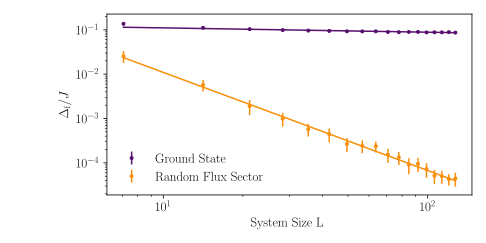
\includegraphics[width=1\textwidth,height=\textheight]{figure_code/amk_chapter/results/fermion_gap_vs_L/fermion_gap_vs_L}
\caption[{Finite Size Scaing of the Fermion Gap}]{Within a flux sector, the fermion gap \(\Delta_f\) measures the energy between the fermionic ground state and the first excited state. This graph shows the fermion gap as a function of system size for the ground state flux sector and for a configuration of random fluxes. We see that the disorder induced by an putting the Kitaev model on an amorphous lattice does not close the gap in the ground state. The gap closes in the flux disordered limit is good evidence that the system transitions to a gapless thermal metal state at high temperature. Each point shows an average over 100 lattice realisations. System size \(L\) is defined \(\sqrt{N}\) where N is the number of plaquettes in the system. Error bars shown are \(3\) times the standard error of the mean. The lines shown are fits of \(\tfrac{\Delta_f}{J} = aL ^ b\) with fit parameters: Ground State: \(a = 0.138 \pm 0.002, b = -0.0972 \pm 0.004\) Random Flux Sector: \(a = 1.8 \pm 0.2, b = -2.21 \pm 0.03\)}
\label{fig:fermion_gap_vs_L}
\end{figure}
}

Next we evaluated the fermionic density of states (DOS), Inverse Participation Ratio (IPR) and IPR scaling exponent \(\tau\) as functions of the vortex density \(\rho\), see \cref{fig:DOS_vs_rho}. This leads to a nice picture of what happens as we raise the temperature of the system away from the gapped, insulating CSL phase. At small \(\rho\), states begin to populate the gap but they have \(\tau\approx0\), indicating that they are localised states pinned to the vortices, and the system remains insulating. At large \(\rho\), the in-gap states merge with the bulk band and become extensive, closing the gap, and the system transitions to the thermal metal phase.

\hypertarget{fig:DOS_vs_rho}{%
\begin{figure}
\centering
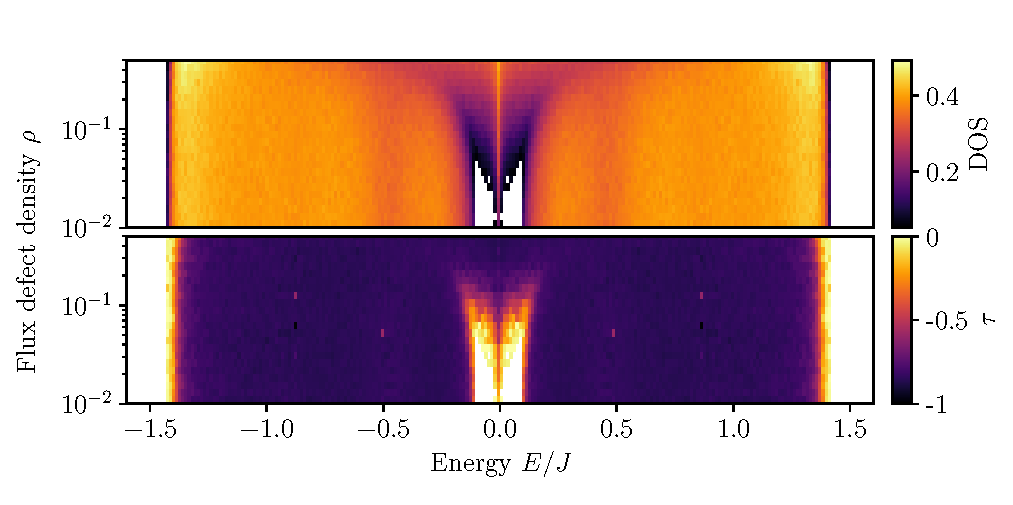
\includegraphics[width=1\textwidth,height=\textheight]{figure_code/amk_chapter/results/DOS_vs_rho/DOS_vs_rho}
\caption[{Transition to a Thermal Metal}]{(Top) Density of states and (Bottom) scaling exponent \(\tau\) of the amorphous Kitaev model as a vortex density \(\rho\) is increased. The scaling exponent \(\tau\) is the exponent with which the inverse participation ratio scales with system size. It gives a measure of the degree of localisation of the states in each \((E/J, \rho)\) bin. At zero \(\rho\) we have the gapped ground state. At small \(\rho\), states begin to populate the gap. These states have \(\tau\approx0\), indicating that they are localised states pinned to fluxes, and the system remains insulating. As \(\rho\) increases further, the in-gap states merge with the bulk band and become extensive, fully closing the gap, and the system transitions to a thermal metal phase.}
\label{fig:DOS_vs_rho}
\end{figure}
}

The thermal metal phase has a signature logarithmic divergence at zero energy and oscillations in the DOS. These signatures can be shown to occur by a recursive argument that involves mapping the original model onto a Majorana model with interactions that take random signs which can itself be mapped onto a coarser lattice with lower energy excitations and so on. This can be repeating indefinitely, showing the model must have excitations at arbitrarily low energies in the thermodynamic limit~\autocite{bocquet_disordered_2000,selfThermallyInducedMetallic2019}.

These signatures for our model and for the honeycomb model are shown in \cref{fig:DOS_oscillations}. They do not occur in the honeycomb model unless the chiral symmetry is broken by a magnetic field.

\hypertarget{fig:DOS_oscillations}{%
\begin{figure}
\centering
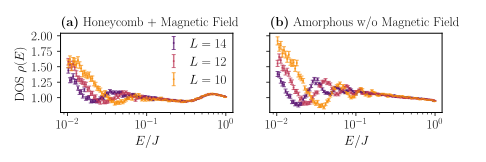
\includegraphics[width=1\textwidth,height=\textheight]{figure_code/amk_chapter/results/DOS_oscillations/DOS_oscillations}
\caption[{Distinctive Oscillations in the Density of States}]{Density of states at high temperature showing the logarithmic divergence at zero energy and oscillations characteristic of the thermal metal state~\autocite{bocquet_disordered_2000,selfThermallyInducedMetallic2019}. (a) shows the honeycomb lattice model in the B phase with magnetic field, while (b) shows that our model transitions to a thermal metal phase without an external magnetic field but rather due to the spontaneous chiral symmetry breaking. In both plots the density of vortices is \(\rho = 0.5\) corresponding to the \(T = \infty\) limit.}
\label{fig:DOS_oscillations}
\end{figure}
}

\hypertarget{sec:AMK-Conclusion}{%
\section{Discussion and Conclusion}\label{sec:AMK-Conclusion}}

\hypertarget{conclusion}{%
\subsection{Conclusion}\label{conclusion}}

In this chapter we have looked at an extension of the Kitaev honeycomb model to amorphous lattices with coordination number three. We discussed a method to construct arbitrary trivalent lattices using Voronoi partitions, how to embed them onto the torus and how to edge-colour them using a SAT solver.

We provided extensive numerical evidence that the ground state flux sector of the model is given by a simply function of the number of sides of each plaquette backed up by an analysis of the energetic finite size effects.

We found two quantum spin liquid phases that can be distinguished using a real-space generalisation of the Chern number. We showed that via finite size scaling that these phases are robustly gapped. The presence of odd-sided plaquettes on these lattices let to a spontaneous breaking of time reversal symmetry, leading to the emergence of a chiral spin liquid phase.

Finally we showed evidence that the amorphous system undergoes an Anderson transition to a thermal metal phase, driven by the proliferation of vortices with increasing temperature.

\hypertarget{discussion}{%
\subsection{Discussion}\label{discussion}}

\textbf{Limits of the ground state conjecture}

We found a small number of lattices for which the ground state conjecture did not correctly predict the true ground state flux sector. I see two possibilities for what could cause this.

Firstly it could be a a finite size effect that is amplified by certain rare lattice configurations. It would be interesting to try to elucidate what lattice features are present when the ground state conjecture fails.

Alternatively, it might be telling that the ground state conjecture failed in the toric code A phase where the couplings are anisotropic. We showed that the colouring does not matter in the B phase. However an avenue that I did not explore was whether the particular choice of colouring for a lattice affects the physical properties in the toric code A phase. It is possible that some property of the particular colouring chosen is what leads to failure of the ground state conjecture here.

\hypertarget{outlook}{%
\subsection{Outlook}\label{outlook}}

This exactly solvable chiral QSL provides a first example of a topological quantum many-body phase in amorphous magnets, which raises a number of questions for future research.

\textbf{Experimental Realisations and Signatures}

The obvious question is whether amorphous Kitaev materials could be physically realised.

Most crystals can as exists in a metastable amorphous state if they are cooled rapidly, freezing them into a disordered configuration~\autocite{Weaire1976,Petrakovski1981,Kaneyoshi2018}. Indeed quenching has been used by humans to control the hardness of steel or iron for thousands of years. It would therefore be interesting to study amorphous version of candidate Kitaev materials~\autocite{trebstKitaevMaterials2022} such as \(\alpha-\textrm{RuCl}_3\) to see whether they maintain even approximate fixed coordination number locally as is the case with amorphous Silicon and Germanium~\autocite{Weaire1971,betteridge1973possible}.

Looking instead at more engineered realisation, metal organic frameworks have been shown to be capable of forming amorphous lattices~\autocite{bennett2014amorphous} and there are recent proposals for realizing strong Kitaev interactions~\autocite{yamadaDesigningKitaevSpin2017} as well as reports of QSL behavior~\autocite{misumiQuantumSpinLiquid2020}.

\textbf{Generalisations}

The model presented here could be generalized in several ways.

First, it would be interesting to study the stability of the chiral amorphous Kitaev QSL with respect to perturbations\textbackslash{} \autocite{Rau2014,Chaloupka2010,Chaloupka2013,Chaloupka2015,Winter2016}.

Second, one could investigate whether a QSL phase may exist for for other models defined on amorphous lattices. For example, in real materials, there will generally be an additional small Heisenberg term \[H_{KH} =  - \sum_{\langle j,k\rangle_\alpha} J^{\alpha}\sigma_j^{\alpha}\sigma_k^{\alpha} + \sigma_j\sigma_k\] With a view to more realistic prospects of observation, it would be interesting to see if the properties of the Kitaev-Heisenberg model generalise from the honeycomb to the amorphous case~{[}\textcite{Chaloupka2010}; \textcite{Chaloupka2015}; \textcite{Jackeli2009}; \textcite{Kalmeyer1989}; \textcite{manousakisSpinTextonehalfHeisenberg1991};{]}.

Finally it might be possible to look at generalizations to higher-spin models or those on random networks with different coordination numbers~\autocite{Baskaran2008,Yao2009,Nussinov2009,Yao2011,Chua2011,Natori2020,Chulliparambil2020,Chulliparambil2021,Seifert2020,WangHaoranPRB2021,Wu2009}

Overall, there has been surprisingly little research on amorphous quantum many body phases albeit material candidates aplenty. We expect our exact chiral amorphous spin liquid to find many generalisation to realistic amorphous quantum magnets and beyond.
